\chapter{Background and Related Work}
\label{chap:background}

This chapter introduces the theoretical foundation and specialized terminology in deep learning and computer vision that underpin this thesis. By defining core architectures, \acrlong{cnn}, \acrlong{rnn} , and transformer variants, the chapter establishes the methodological basis for experiments. Next, it outlines standard evaluation metrics, \acrfull{map} and temporal intersection‑over‑union (IoU), to ensure reproducible performance assessment. The chapter then examines advanced video‑analysis methodologies, including spatiotemporal convolutions, state‑space models, and masked autoencoder frameworks. Finally, it reviews recent football‑event‑spotting research—such as COMEDIAN and VideoMAMBA, to identify specific limitations that motivate our proposed approach. % ait

\section{Football Analytics}
\label{sec:football_analytics}

\subsection{Continuous Nature of Football}
Football presents a continuous, dynamic domain unlike sports with discrete plays such as baseball or cricket. For example, a goalkeeper’s pass occurs during uninterrupted action and results in numerous possible temporal sequences and starting conditions. This constant flow challenges both event-based models, which identify individual occurrences and sequence-based models—which analyze ordered temporal inputs. Consequently, traditional discrete frameworks must be extended to preserve contextual information across continuous match sequences. % ait

\subsection{Data Sources and Key Metrics}
Football analytics rely on two primary data streams:

\begin{figure}
    \centering
    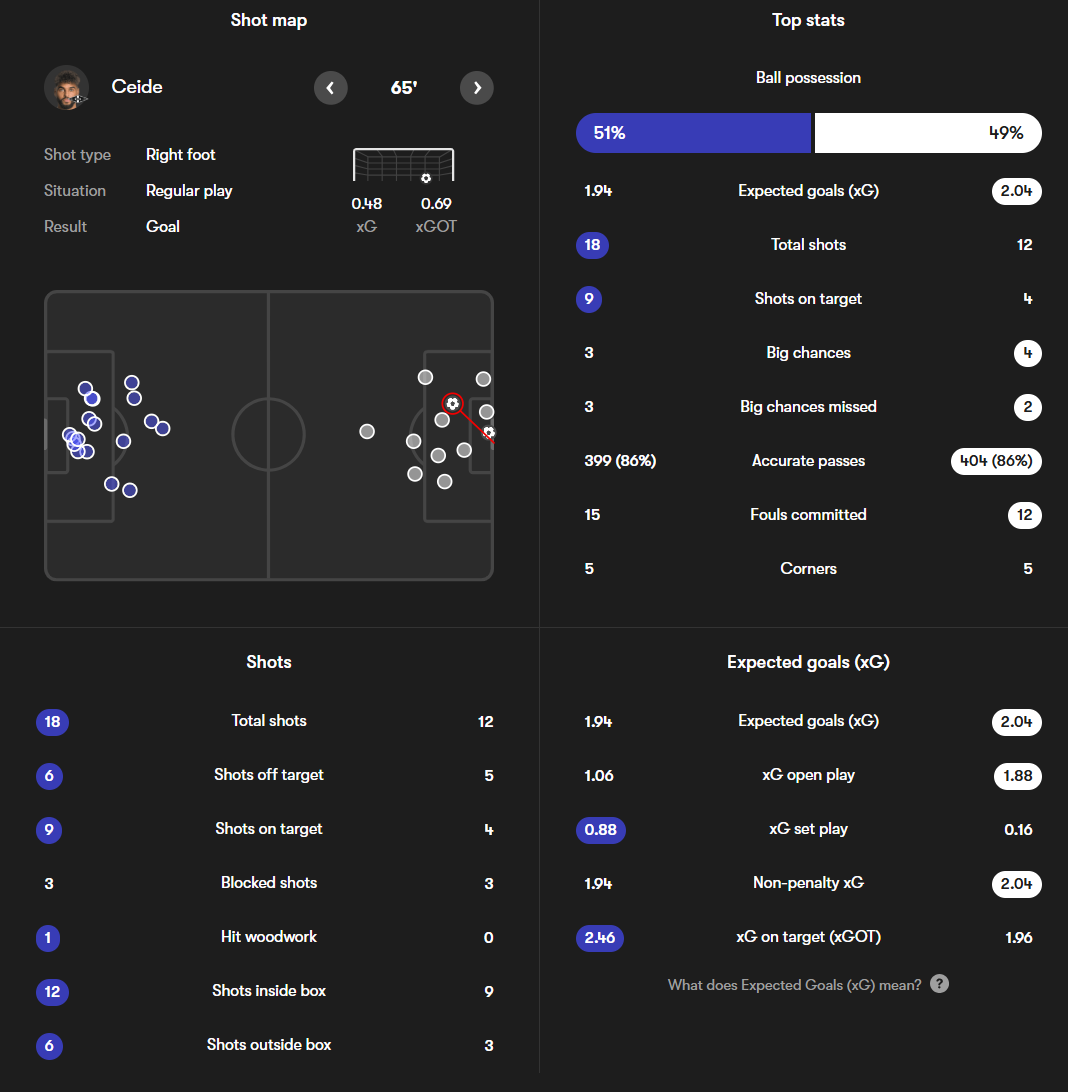
\includegraphics[width=0.5\linewidth]{figures/fotmob_rbk.png}
    \caption{Commercially available stats from a football game. Retrieved from FotMob\cite{fotmob_game}.}
    \label{fig:fotmob_stats}
\end{figure}

\begin{itemize}
    \item Event data: manually or commercially annotated discrete occurrences (passes, shots, corners).
    \begin{itemize}
        \item \acrfull{xg}: estimates shot quality using spatial and contextual features with XGBoost trained on large historic datasets \cite{mead_xg_2023}.
        \item Set pieces (corners, free kicks): naturally bounded events suitable for end-to-end predictive models.
        \item \autoref{fig:fotmob_stats} shows a selection of commercially available statistics. 
    \end{itemize}
    \item Tracking data: high-frequency player trajectories from GPS vests or manual optical systems.
    \begin{itemize}
        \item Physical metrics: distance covered, top speed, accelerations for workload monitoring and injury risk assessment \cite{hennessy_gps_tracker_2018}.
    \end{itemize}
\end{itemize}

\textcite{wang_tactic_ai_2024} applies deep graph neural networks to corners, a discrete sub-event of play. They deliver strong predictive and generalizable performance and have helped Liverpool FC succeed. % ait

\section{Deep Learning}
\label{sec:deep_learning}

Deep learning comprises multilayer neural networks that automatically learn hierarchical data representations. By contrast, classical methods rely on handcrafted features; deep architectures instead discover interesting patterns from raw inputs. They stack linear transformations and non‑linear activations to extract meaningful features at each layer \cite{lecun_deep_learning_2015}. 
Early layers capture low‑level primitives, while deeper layers combine these primitives into high‑level concepts. Model training uses backpropagation to compute loss gradients with respect to millions of parameters. % to cv related, the second part?

\subsection{Forward pass}
For a network with two hidden layers, the forward pass can be written as:
\begin{align}
z^{(1)} &= W^{(1)} x + b^{(1)}, & y^{(1)} &= f\bigl(z^{(1)}\bigr), \\
z^{(2)} &= W^{(2)} y^{(1)} + b^{(2)}, & y^{(2)} &= f\bigl(z^{(2)}\bigr), \\
z^{(3)} &= W^{(3)} y^{(2)} + b^{(3)}, & \hat{y} &= g\bigl(z^{(3)}\bigr).
\end{align}
Here, \(x\in\mathbb{R}^d\) is the input, \(W^{(l)},b^{(l)}\) are weights and biases at layer \(l\), \(f(.)\) is an activation function (e.g. ReLU). Figure~\ref{fig:forward_pass} illustrates these computations. In the case of a classification task, \(g\) is the output activation (e.g. softmax) and \(\hat{y}\) is the predicted class.

\begin{figure}[ht]
    \centering 
    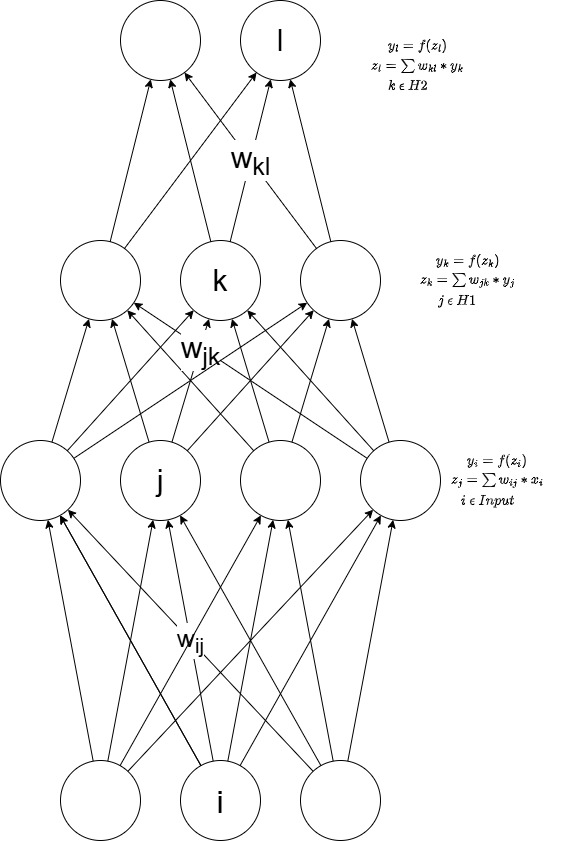
\includegraphics[width=0.6\linewidth]{figures/neural_net.jpg}
    \caption{Feedforward pass of a neural network with two hidden layers.} % there was an equation here but it is better in the figure?
    \label{fig:forward_pass}
\end{figure}

\subsection{Backward pass}
Training minimizes a loss \(E(\hat y, y^\star)\), using e.g. cross-entropy. Gradients are computed via the chain rule:
\begin{align}
\delta^{(3)} &= \frac{\partial E}{\partial z^{(3)}}
= \frac{\partial E}{\partial \hat y}\odot g'\bigl(z^{(3)}\bigr),\\
\delta^{(l)} &= \frac{\partial E}{\partial z^{(l)}}
= \bigl(W^{(l+1)\top}\delta^{(l+1)}\bigr)\odot f'\bigl(z^{(l)}\bigr),
\quad l=2,1.
\end{align}
Weight and bias gradients follow:
\begin{align}
\nabla_{W^{(l)}}E &= \delta^{(l)}\,y^{(l-1)\top}, &
\nabla_{b^{(l)}}E &= \delta^{(l)},
\end{align}
with \(y^{(0)}\equiv x\). Figure~\ref{fig:backward_pass} shows the backpropagation flow.
\unsure{bad caption on figure below?}
\begin{figure}[ht]
    \centering
    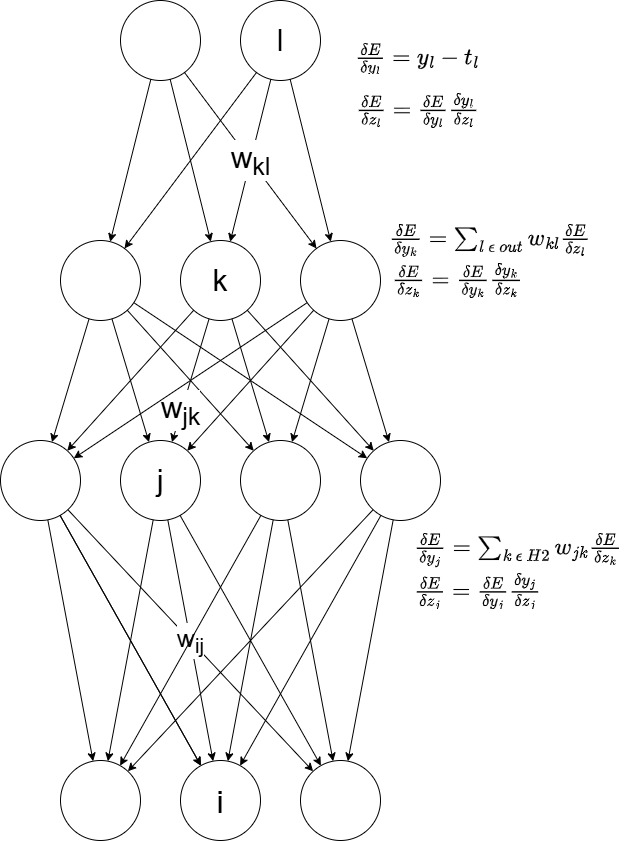
\includegraphics[width=0.6\linewidth]{figures/neural_net_back_prop.jpg}
    \caption{The equations compute the backward pass.} 
    \label{fig:backward_pass}
\end{figure}

\subsection{Optimization}
Parameters are updated with stochastic gradient descent (SGD) or adaptive variants (Adam, RMSProp). For learning rate \(\eta\),
\[
W^{(l)} \leftarrow W^{(l)} - \eta\,\nabla_{W^{(l)}}E,
\quad
b^{(l)} \leftarrow b^{(l)} - \eta\,\nabla_{b^{(l)}}E.
\]
Regularization techniques such as weight decay, dropout and batch normalization further improve generalization and training stability \cite{ioffe_batch_2015}.

\subsection{Convolutions}

Convolutions learn small filters that slide over the input to detect local features in space (and time). Each filter is a small tensor of weights that computes a weighted sum plus a bias at every position. By sharing the same weights across all locations, convolutions capture patterns such as edges, textures, or motion.  

In the most basic scenario, when there is a layer with input dimensions of \( (N, C_{in}, H, W)\) and output dimensions of \( (N, C_{out}, H_{out}, W_{out})\), the output can be accurately described as follows:

\[out(N_i, C_{out_j}=bias(C_{out_j})+\sum_{k=0}^{C_{in}-1}weight(C_{out_j},k)\star input(N_i,k)\]

In this expression, the symbol \(\star\) represents the valid 2D cross-correlation operation. Here, \textit{\textbf{N}} refers to the batch size, \textit{\textbf{C}} indicates the number of channels, \textit{\textbf{H}} represents the height of the input planes measured in pixels, and \textit{\textbf{W}} denotes the width measured in pixels. \unsure{this is from pytorch, but everyone says the same, should I cite?}

Key components:
\begin{itemize}
    \item \textbf{Stride}, \textbf{padding}, and \textbf{dilation} control the receptive field and output resolution.
    \item \textbf{Pooling} (max or average) reduces spatial dimensions and enforces translational invariance.
    \item \textbf{Batch normalization} stabilizes learning by normalizing activations per mini-batch.
    \item Non-linear activations (ReLU, LeakyReLU, etc.). \unsure{pointless and redundant?}
\end{itemize}

\begin{figure}
    \centering
    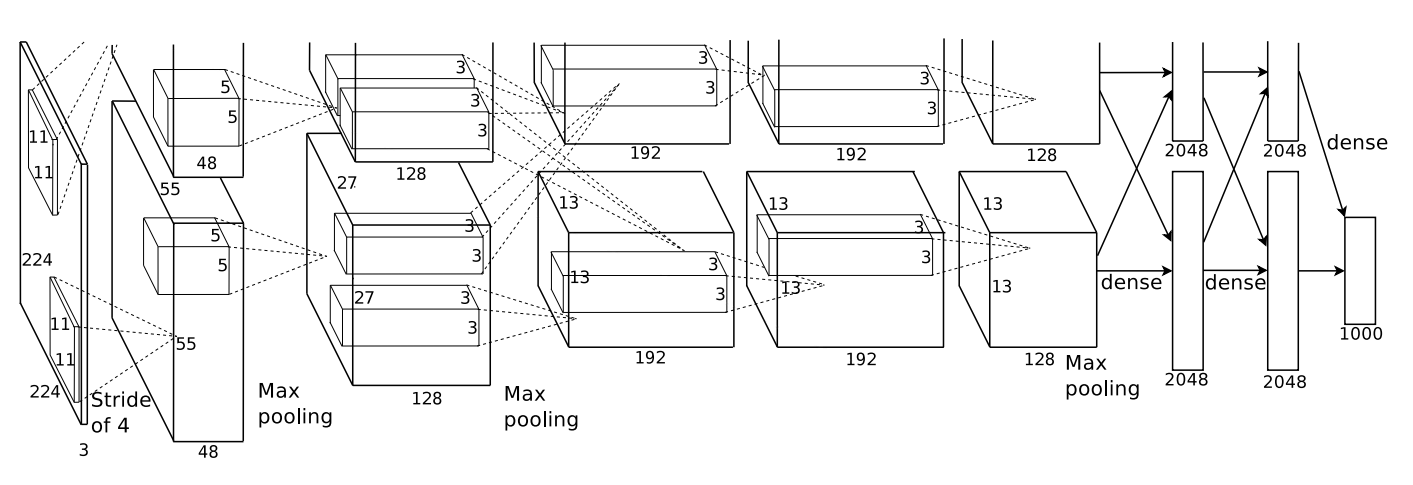
\includegraphics[width=1\linewidth]{figures/alexnet.png}
    \caption{An illustration of the architecture of AlexNet. One GPU runs the layer-parts at the top of the figure while the other runs the layer-parts at the bottom. The figure and caption is Figure 2 in the released paper by \textcite{krizhevsky_alexnet}.}
    \label{fig:alexnet}
\end{figure}

Stacking multiple convolution–activation–pooling blocks builds hierarchical feature representations, from edges and textures in early layers to object parts in deeper layers \cite{lecun_deep_learning_2015}. \autoref{fig:alexnet} shows how \textcite{krizhevsky_alexnet} designed AlexNet in 2012 with alternating convolution and pooling layers. Residual connections \cite{he_deep_residual_2015} further ease training in very deep networks by learning residual mappings. An example of a residual block is shown in \autoref{fig:res_connection}. Architectures such as Inception \cite{szegedy_going_2014}, MobileNet (depthwise separable convolution) \cite{howard_mobilenets_2017} and EfficientNet (compound scaling) \cite{tan_efficientnet_2020} optimize accuracy–efficiency trade-offs in image tasks. 

\begin{figure}
    \centering
    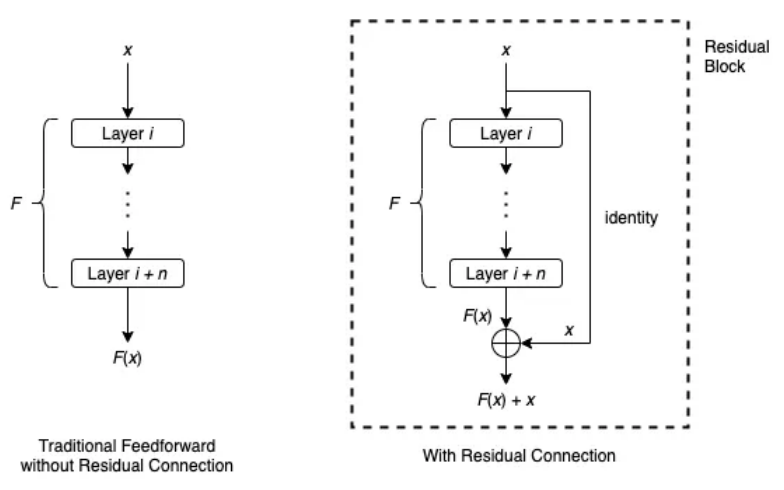
\includegraphics[width=0.5\linewidth]{figures/res_connection.png} 
    \caption{Residual block. Created by \textcite{wong_what_is_residual_2022}. }
    \label{fig:res_connection}
\end{figure}

In the video domain, spatiotemporal convolutions extend the same principles along time.  Early 3D \acrshort{cnn}s \cite{tran_learning_2015} apply cubic kernels to capture motion, but suffer from high computational cost.  The (2+1)D decomposition \cite{tran_2_plus_1_convolution} splits 3D kernels into separate spatial and temporal convolutions, improving the optimization.  The Inflated 3D \acrshort{cnn} (I3D) \cite{carreira_2017_i3d_quo_vadis} “inflates” pretrained 2D filters into the time dimension. This creates a balance between efficiency and representation.

Further advances address long-range temporal modeling:
\begin{itemize}
    \item SlowFast networks \cite{feichtenhofer_slowfast_2019} use a dual-pathway: a \emph{Slow} branch at low frame rate for semantics and a \emph{Fast} branch at high frame rate for motion.  
    \item Temporal Shift Module (TSM) \cite{lin_temporal_shift_2019} achieves temporal modeling by shifting feature channels across frames with zero extra parameters.  
    \item X3D \cite{feichtenhofer_x3d_2020} systematically expands 2D image models into efficient, scalable 3D architectures by progressive width, depth and resolution scaling.
\end{itemize}

Despite their locality bias, \acrshort{cnn}-based video models remain foundational building blocks in modern action-recognition frameworks, often combined with non-local blocks or attention to capture global spatiotemporal dependencies.
\info{another paragraph with a different approach is below} \info{Another angle of writing about convolutions are deleted 2nd may 9.26, can be found in overleaf history}


\subsection{Recurrent Neural Nets}

\acrfull{rnn} are a class of deep learning models designed to handle sequential data. \acrshort{rnn}s keep a memory of previous inputs. Unlike tradtional feedforward networks, for example \acrshort{cnn}s and neural nets, \acrshort{rnn}s use feedback loops that allows information to exist over multiple time steps. \unsure{Do I say the same sentence twice here?} This makes \acrshort{rnn}s useful for tasks requiring temporal dependencies, such as natural language processing, speech recognition and time-series forecasting\cite{ibm_rnn_2025}. In the context of \acrfull{cv}, \acrshort{rnn}s have been applied for applications such as image captioning or video analysis. \unsure{Is it better to write in present?}

Standard \acrshort{rnn}s suffer from the vanishing gradient problem. The issue is due to repeated multiplication of small gradient values during backpropagation through time. This leads to diminishing updates in early layers. \acrfull{lstm} is one solution to this problem \cite{bhogal_human_2023, kumar_human_2023, mahaseni_spotting_2021}.The other widespread solution is the \acrfull{gru} \cite{giveki_human_2024,li_oarnet_2024,yu_i3d_2023}. 

\acrlong{lstm} introduce memory cells. The cells are equipped with input, forget and output gates. \acrshort{lstm}s come with increased efficiency and increased complexity. On small datasets \acrshort{lstm}s are prone to overfitting. 

\acrlong{gru}s use a reset gate and an update gate to maintain or discard information. It has fewer parameters than an \acrshort{lstm}, which makes them more computationally efficient while addressing the vanishing gradient problem. \acrshort{gru} are particularly attractive in scenarios with limited resources. 

\acrshort{rnn}-based architectures are used in video analysis models to capture temporal dependencies, like \textcite{bhogal_human_2023}. Although a historically popular resource for sequential data processing, transformer models have led to a decline in their usage. However, they remain relevant in contexts where step-by-step recurrence and memory provide distinct advantages\cite{ibm_rnn_2025}.

\subsubsection{Bi-Directional Layers}
\label{ssec:bi_directional_layers}

Bi-directional recurrent layers combine two parallel LSTM networks to capture both past and future context in a sequence \cite{radhakrishnan_bi_lstm_2023, bhogal_human_2023}. One LSTM processes the input in its original order (forward pass), while the other processes it in reverse (backward pass). At each time step \(t\), the hidden states from both directions are concatenated to form a richer representation of the data:

\[
h_t = \bigl[\,\overrightarrow{h}_t;\,\overleftarrow{h}_t\bigr].
\]

In the context of football analytics, this approach is useful because events (e.g.\ goals, passes) often depend on both preceding and succeeding actions on the field. By integrating information from before and after a given frame, bi-directional layers can improve the accuracy of sequence predictions. The main trade-off is that they require roughly twice the number of parameters and incur longer training and inference times compared to unidirectional models.


\subsection{Vision Transformers}
\label{ssec:vision_transformers}

\acrfull{vit} adapt the transformer architecture \cite{vaswani_attention_2017} \change{Does transformers by themselves deserve a section?} to images by splitting each image into $P\times P$ patches, projecting them to $D$-dimensional embeddings, and adding positional encodings \cite{dosovitskiy_image_transformer_2021}. Given an image of size $H\times W$, one obtains
\[
\mathbf{x}_0 = [x_{\text{cls}};\,z_1,\dots,z_N] + E_{\text{pos}},
\]
$x_{\text{cls}}$ is a learnable classification token, and $E_{\text{pos}}\in\mathbb{R}^{(N+1)\times D}$ are positional embeddings, where $N=(H/P)\,(W/P)$,. The sequence is processed by $L$ identical blocks of multi-head self-attention (MSA) and feed-forward networks (FFN):
\begin{align*}
y^l &= \mathrm{MSA}\bigl(\mathrm{LN}(x^{l-1})\bigr) + x^{l-1},\\
x^l &= \mathrm{FFN}\bigl(\mathrm{LN}(y^l)\bigr) + y^l,\quad l=1,\dots,L.
\end{align*}
\info{Math from top of page 4 on \textcite{dosovitskiy_image_transformer_2021}}

TimeSformer \cite{bertasius_timesformer_2021} extends ViT to video by factorizing self-attention into separate spatial and temporal modules, reducing complexity from $\mathcal{O}\bigl((TN)^2\bigr)$ to $\mathcal{O}(T^2N + N^2T)$. Formally, with tokens $z_{t,n}$ for frame $t$ and patch $n$,
\[
\mathrm{Attn}(Z)
= \mathrm{Softmax}\!\bigl(Q_sK_s^\top/\sqrt{D}\bigr)V_s
+ \mathrm{Softmax}\!\bigl(Q_tK_t^\top/\sqrt{D}\bigr)V_t.
\]

VViT \cite{arnab_vvit_2021} further improves video classification by combining factorized attention with multi-scale patch embeddings, achieving state-of-the-art results on multiple benchmarks.


Limitations of vision transformers include:
\begin{itemize}

    \item High data requirements—performance degrades on small or specialized datasets.  
    \item Computational cost—quadratic scaling with sequence length impacts memory and runtime.  
    \item Model complexity—large parameter counts increase overfitting risk \cite{lee_enhancing_mamba_s6_2024}.
\end{itemize}

% \acrfull{sam} \cite{kirillov_segment_2023} employs a ViT backbone augmented with mask-attend-segment heads to enable promptable segmentation in both images. \acrlong{sam}-2 \cite{ravi_sam_nodate} extended its use to videos. In football analytics, transformer-based approaches such as COMEDIAN \cite{denize_comedian_2024} and real-time optimizations \cite{sarraf_optimal_2023} demonstrate strong performance in action-spotting tasks.


\subsubsection{META Segment Anything Model 2}
\label{ssec:meta_sam2}

The Segment Anything Model (SAM) was first introduced by Kirillov et al.\ \cite{kirillov_segment_2023} in 2023 as a promptable, foundation segmentation model.  Its core design splits the task into three components:
\begin{itemize}
    \item \textbf{Image Encoder:} A vision transformer (ViT) pretrained on masked autoencoding, which produces dense feature maps for any input image.
    \item \textbf{Prompt Encoder:} A lightweight module that maps interactive prompts (points, bounding boxes or free‐form masks) into positional embeddings.
    \item \textbf{Mask Decoder:} A small transformer that fuses image and prompt embeddings to output segmentation masks at multiple scales.
\end{itemize}
SAM was trained on the enormous SA‑1B dataset (over 11 M images and 1.1 B masks) in a semi‑automated pipeline, yielding strong zero‑shot performance across diverse domains without any finetuning.

Building on this success, Ravi et al.\ \cite{ravi_sam_nodate} proposed \emph{SAM‑2} (sometimes called Video \acrshort{sam}), which extends \acrshort{sam} to sequential video data via a \emph{memory‐augmented attention} mechanism:
\begin{itemize}
    \item \textbf{Frame‐wise Encoding:} Each video frame is encoded by the same ViT backbone used in image \acrshort{sam}.
    \item \textbf{Memory Attention:} A cross‐frame attention layer that retains a compact set of “memory tokens” summarizing past masks, enabling consistent tracking of object masks over time.
    \item \textbf{Interactive Prompts in Video:} Mouse clicks and bounding‐box prompts can be applied on any frame, and propagated forward or backward via the memory bank.
\end{itemize}
The authors also released SA‑V, a large video‑segmentation dataset with millions of frame‐mask pairs, demonstrating that \acrshort{sam}‑2 achieves near real‐time inference (15–30 fps) and high temporal consistency on common benchmarks.

Together, the original \acrshort{sam} and its video‐centric successor exemplify a new paradigm in segmentation: a single, promtable\unsure{promtable or promtable?} transformer that can be deployed off‐the‐shelf, adapted to novel objects or domains with minimal human guidance, and extended from static images to dynamic scenes. 

\improvement{To increase readability I this section needs more figures, not only here}
\subsection{State‐Space Models}
\label{ssec:state_space_models}

\acrfull{ssm} offer a continuous‐time representation of sequential data via a latent state \(h(t)\in\mathbb{R}^N\):
\begin{align}
    \frac{\mathrm{d}h(t)}{\mathrm{d}t} &= A\,h(t) + B\,x(t),  \label{eq:ssm_continuous1}\\
    y(t) &= C\,h(t),                                    \label{eq:ssm_continuous2}
\end{align}
where \(x(t)\in\mathbb{R}^d\) is the input, \(y(t)\in\mathbb{R}^m\) the output, and \(A\in\mathbb{R}^{N\times N}, B\in\mathbb{R}^{N\times d}, C\in\mathbb{R}^{m\times N}\) are learned parameters.  Discretizing these equations with step size \(\Delta\) yields
\begin{align}
    \bar A &= \exp(\Delta\,A), 
    & 
    \bar B &= \bigl(\exp(\Delta\,A)-I\bigr)A^{-1}B,\\
    h_k &= \bar A\,h_{k-1} + \bar B\,x_k, 
    &
    y_k &= C\,h_k,
    \quad k=1,2,\dots
\end{align}
\unsure{Do I have to reference equations in the same way figures must be referenced in a text}
VideoMamba \cite{li_videomamba_2024} builds on this framework with a \emph{Selective Scan} (\acrshort{s6}) core.  Its parameters \((\Delta, A,B,C)\) control:
\begin{itemize}
    \item \(\Delta\): temporal resolution of the recurrence,
    \item \(A\): continuous dynamics matrix,
    \item \(B,C\): input and output mappings.
\end{itemize}

By preserving a compact hidden state, Mamba approximates long‐range dependencies akin to self‐attention but with only \(\mathcal{O}(L)\) time/memory cost rather than \(\mathcal{O}(L^2)\).  

VideoMAMBA extends \acrshort{s6} to spatiotemporal video features: each frame is first embedded (e.g.\ via convolutional or patch‐based encoders) into \(x_k\), then processed through the discrete SSM along the temporal dimension.  Prior studies \cite{lee_enhancing_mamba_s6_2024, li_videomamba_2024} report that VideoMAMBA matches transformer‐based action recognition on common benchmarks while reducing inference overhead.

This thesis applies the VideoMAMBA suite to a newly collected football video dataset to evaluate its event‐spotting performance (see Chapter~\ref{chap:experiments}). The results demonstrate that VideoMAMBA not only achieves competitive accuracy but also delivers substantial gains in inference speed and memory efficiency, confirming the practicality of state‐space models for large‐scale video analytics. \unsure{Remove this paragraph? Move to intro?}


\subsection{Training Strategies}
\label{ssec:training_stratergies}
\subsubsection{Learning Paradigms}
A model must be trained on domain‑specific data to achieve its full potential. Training algorithms for artificial neural networks (ANNs) can be broadly grouped into four categories: supervised learning, unsupervised learning, self‑supervised learning, and reinforcement learning. This thesis focuses on supervised and unsupervised learning, which are detailed below.\improvement{Replace this thesis }

\paragraph{Supervised Learning}
In supervised learning, models are trained on labeled data comprising input–output pairs \((x_i, y_i)\). The objective is to learn a mapping that generalizes to unseen data. In this thesis\improvement{"this thesis"}, supervised labels include bounding‑box coordinates of players and the ball in football match images, and the model is tasked with detecting these objects in new footage. Gradient descent optimizes the parameters \(\theta\) by minimizing a loss function \(J(y_i, \hat y_i)\):  
\[
\theta \leftarrow \theta - \eta \,\nabla_{\theta}J\bigl(y_i,\hat y_i\bigr),
\]
where \(\eta\) is the learning rate. Updates continue over the dataset until a stopping condition is met (e.g., maximum epochs, target loss, or early stopping).

\paragraph{Unsupervised Learning}
Unsupervised learning discovers structure from unlabeled data without explicit targets. Common tasks include clustering, association rule mining, and dimensionality reduction. \improvement{does this need to be longer?}\unsure{should I write just about supervised learning?}

\subsubsection{Masking}

In an encoder–decoder masking setup, the input video frames are first tokenized into spatio-temporal patches. A binary mask tensor \(M\in\{0,1\}^{T\times H\times W}\) with masking ratio \(r\) is generated, where
\[
\sum_{t,h,w} M_{t,h,w} = r\,T\,H\,W.
\]
The visible patches \(x_\text{vis}\) are obtained by
\[
x_\text{vis} = x \,\odot\,(1 - M)\,,
\]
and fed into a lightweight transformer encoder \(E\). The decoder \(D\) takes the encoder output plus positional embeddings and mask tokens, and attempts to reconstruct the original video:
\[
\hat{x} = D\bigl(E(x_\text{vis}),\,\text{mask\_tokens}\bigr).
\]
The model is trained to minimize the reconstruction loss only over masked positions:
\[
\mathcal{L} \;=\; \bigl\lVert\,M \,\odot\,(x - \hat{x})\bigr\rVert_2^2.
\]
Different masking strategies can be used:
\begin{itemize}
    \item Random tube masking: mask entire temporal tubes to encourage long-range dynamics learning.
    \item Block spatial masking: mask contiguous patches in each frame.
    \item Uniform patch masking: randomly mask individual patches across space and time.
\end{itemize}
High masking ratios (e.g.\ 75–90\%) force the encoder to capture global context, while the decoder reconstructs fine-grained details from a compact latent code. This approach underlies VideoMAE and similar masked autoencoder variants for self-supervised video representation learning.


Encoding and masking techniques are used with video data because of their inherent large size. Encoding encapsulates the process of compressing video files to reduce size while keeping a satisfactory quality. Video masking is the technique used to discard uninteresting regions and patches to focus on more meaningful features. This motivates the model to learn meaningful representations, rather than predicting based on redundant data \cite{tong_videomae_2022}. The most prominent masking variant used on \acrshort{sota} benchmarks on Papers with Code' in the category \textit{Action Recognition}\footnote{\url{https://paperswithcode.com/task/action-recognition-in-videos}} is the VideoMAE V2 \cite{wang_videomae_2023} and its highly related InternVideo2 \cite{wang_internvideo2_2024}. 

\textcite{tong_videomae_2022} address the problem of training video transformers from scratch. The aim is to use self-supervised learning to capture meaningful representations which enables the model to decode data into the original representations. The contributions of the masked autoencoder \cite{tong_videomae_2022} are the ability to train \acrshort{vit}s on smaller datasets. VideoMAE \cite{tong_videomae_2022} also tackle the problems of temporal relations in video-data and suggests a high masking ratio. VideoMAE-V2 \cite{wang_videomae_2023} improves the VideoMAE-models training time. It is still a very computationally expensive approach. 

\subsubsection{VideoMAE-V2}
\label{sssec:videomae_v2}

\info{I want to have this section because it is relevant for my feature extraction. But I see it overlapps with general VideoMAE}
VideoMAE‑V2 \cite{wang_videomae_2023} is a self‑supervised masked autoencoder designed specifically to preprocess and compress large‑scale video data before downstream experiments. Building on the original VideoMAE, it introduces a dual‑stage masking schedule: 
\begin{itemize}
    \item \emph{Sparse spatiotemporal masking} in early epochs to encourage global context learning over long clips,
    \item \emph{Dense tube masking} in later epochs to refine local motion representations.
\end{itemize}
Each frame is first partitioned into non‑overlapping $P\times P$ patches and tokenized; a binary mask tensor $M\in\{0,1\}^{T\times H/P\times W/P}$ with masking ratio up to 90\% is then generated according to the dual schedule. The visible tokens $x_{\rm vis}=x\odot(1-M)$ are encoded by a standard ViT backbone, while a lightweight three‑layer transformer decoder reconstructs only the masked patches. 

By dynamically varying the masking granularity, VideoMAE‑V2 achieves:
\begin{itemize}
    \item 2× faster convergence compared to VideoMAE,
    \item linear scaling to billion‑parameter models,
    \item robust transferability across action recognition, temporal localization and segmentation tasks.
\end{itemize}

In the preprocessing pipeline (Chapter \ref{chap:experiments}), I apply VideoMAE‑V2 to each football clip to extract a compact latent representation. These features, computed once offline, reduce storage requirements and enables efficient training and evaluation of downstream event‑spotting.


\subsubsection{Knowledge Distillation}
\label{sssec:knowledge_distillation}

Knowledge distillation trains a compact \emph{student} model to mimic a larger, pre-trained \emph{teacher} model \cite{denize_comedian_2024, li_videomamba_2024, bose_soccerkdnet_2023}. By matching the teacher’s softened output distribution (using a temperature-scaled softmax), the student can achieve similar accuracy with far fewer parameters. This reduction in size and computation is particularly valuable for video models with high inference cost.

However, distillation also has limitations:
\begin{itemize}
    \item A weak teacher leads to a weak student—distillation cannot exceed the teacher’s performance.
    \item Training both teacher and student increases total computational cost.
    \item Some fine-grained knowledge may not transfer fully, which can hurt the student’s generalization on new data.
\end{itemize}


\section{Computer Vision} 
\label{sec:computer_vision}

\acrfull{cv} is a subset of machine learning that focuses on letting computers interpret and understand digital images and videos. The aim of \acrlong{cv} is to enable computers to see. Some tasks relating to computer vision, extracted from Papers with Code\footnote{\url{https://paperswithcode.com/datasets}}, are Action Recognition, Object Detection, Semantic Segmentation, Classification and Question Answering. 

\subsection{Hand-Crafted methods}

\begin{figure}
    \centering
    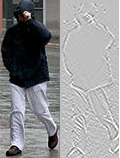
\includegraphics[width=0.5\linewidth]{figures/Pedestrian_gradient.jpg}
    \caption{An image of a pedestrian and his gradient}
    \label{fig:pedestrian_gradient}
\end{figure}

Before the rise of deep learning, early computer vision research predominantly relied on manually engineered features. One of the influential approaches was the \acrfull{hog} introduced by \textcite{dalal_histogram_of_gradients}. This method was designed to detect humans in static images by partitioning an image into small regions and computing gradient directions within each patch, ultimately assembling these measurements into a descriptive feature vector. \autoref{fig:pedestrian_gradient} visualizes the gradient vectors. In a similar fashion, action recognition in videos was addressed through the Histogram of Flow\cite{dalal_histogram_of_flow}. This technique extends the \acrshort{hog} concept by calculating gradient descriptors at each frame, capturing motion information through the analysis of optical flows. Then combining these per-frame descriptors into a representation that encapsulates temporal dynamics. \unsure{The image is from wikipedia, but they do not provide any source for it.}

Despite the innovation these approaches brought to early computer vision, their limitations soon became apparent. The reliance on accurate hand-crafted features often led to challenges in scaling to complex scenarios and achieving generalization. With the arrival of deep learning and its ability to learn hierarchical, data-driven representations, these manual methods have been largely outpaced. 

\subsection{Skeleton and Posture Estimation}
\label{ssec:skeleton_posture_estimation}

Skeleton and posture estimation techniques recover 2D or 3D joint coordinates from video frames to model player kinematics and pose dynamics \cite{elaoud_skeleton-based_2020, wang_skeleton_two-stream_2023, reilly__skeleton_just_pi_2023}. Common pipelines include:
\begin{itemize}
    \item Top-down methods: detect each player via bounding boxes, then apply a single-person pose estimator.
    \item Bottom-up methods: predict all joint candidates first and group them into skeletons.
    \item Graph-based models: use spatial–temporal graph convolutional networks (ST-GCN) to capture joint correlations over time\cite{yan_spatial_temporal_graph_convolutional_2018}.
\end{itemize}
These approaches enable extraction of features such as joint angles, stride length and posture transitions for performance analysis and injury risk assessment. In football scenarios, however, they face:
\begin{itemize}
    \item Severe occlusions and player overlaps in crowded penalty areas.
    \item Varying camera angles, resolutions and lens distortions.
    \item Fast motions causing motion blur and tracking drift\cite{survey_of_survey}.
\end{itemize} 
% Recent advances leverage multi-view fusion, temporal consistency constraints and weakly supervised learning to enhance robustness under challenging match conditions.


\section{Datasets}
\label{sec:datasets}


\subsection{SoccerNet‑V2}
\label{ssec:soccernet}

The SoccerNet‑V2 dataset \cite{deliege_soccernet-v2_dataset_2021} contains video recordings of 7 professional football matches with fine‑grained annotations for 12 action classes. It provides:
\begin{itemize}
    \item 7 full matches (90 min each) at 25 fps.
    \item Time‑stamped action labels for spotting tasks.
    \item Team annotations for each event.
    \item Publicly accessible via HuggingFace\footnote{\url{https://huggingface.co/datasets/SoccerNet/SN-BAS-2025}}.
    \item The twelve football event classes:
        \begin{center}
            \begin{tabular}{llll}
                Pass & Drive & Header & High Pass \\
                Out & Cross & Throw In & Shot \\
                Ball Player Block & Player Successful Tackle & Free Kick & Goal
            \end{tabular}
        \end{center}
    \item An action approximately every 3 seconds. 
\end{itemize}

The original SoccerNet dataset contains the recording of 500 games with 17 action classes. 


\subsection{THUMOS'14}
\label{ssec:thumos}

The THUMOS'14 dataset \cite{dataset:thumos} comprises:
\begin{itemize}
    \item 20 action classes in sports and daily activities.
    \item 213 untrimmed videos for temporal detection.
    \item Predefined train/val/test splits for benchmarking.
\end{itemize}

\section{Problem Formulation}
\label{sec:problem_formulation}
Ball action spotting requires detecting and classifying discrete ball‐related events in continuous football video streams. Given a video sequence \(V\) of \(T\) frames \(\{x_t\}_{t=1}^T\), the task is to predict a set of event timestamps \(\{\hat t_j\}\) and corresponding class labels \(\{\hat c_j\}\) over the 12 predefined action categories. Each event is annotated by a single timestamp, and—unlike the original SoccerNet Spotting Challenge—the new dataset has a higher density of actions per minute, placing greater demands on temporal precision.

\subsection{Action Spotting vs. Action Localization}
Action spotting casts each event as a single instant in time, reducing annotation to one timestamp per occurrence. By contrast, action localization requires predicting both start and end times for each action interval and is typically evaluated with temporal \acrfull{iou} metrics. Spotting simplifies supervision and evaluation (via tolerance windows around true timestamps), but it also challenges models to resolve events occurring in close temporal proximity without relying on segment boundaries.

\subsection{Temporal vs. Spatiotemporal Tasks}
Temporal event spotting focuses solely on “when” an action occurs, using global frame or clip‐level features. Spatiotemporal tasks, in comparison, demand joint localization in time and space (e.g.\ frame‐level bounding boxes). The SoccerNet challenge remains in the temporal domain. 

\subsection{Notation and Task Definition}
Let
\begin{itemize}
    \item \(V = \{x_t\}_{t=1}^T\) Let be an input video of \(T\) frames,  
    \item \(\mathcal{C} = \{1,\dots,12\}\) the set of action classes,  
    \item \(\mathcal{Y} = \{(t_i,c_i)\}_{i=1}^N\) the ground‐truth annotations (timestamp \(t_i\), class \(c_i\)),  
    \item \(\hat{\mathcal{Y}} = \{(\hat t_j,\hat c_j,\hat s_j)\}_{j=1}^M\) the model’s predictions with confidence scores \(\hat s_j\).  
\end{itemize}
A prediction \((\hat t_j,\hat c_j)\) is correct if \(\hat c_j=c_i\) and \(|\hat t_j - t_i|\le\Delta\), where \(\Delta\) is a tolerance window (\ 1s). We evaluate performance by \acrfull{map} over all classes under the chosen \(\Delta\).  \unsure{"we" feels right but also wrong, but "i" feels worse}


\section{Temporal Modeling Techniques}\unsure{Should I remove this section}
\label{sec:temporal_models}

Temporal modeling techniques aim to capture motion and long‐range dependencies across video frames. Common approaches include: \unsure{is this redundant}

\paragraph{\acrfull{rnn}}  
LSTM and GRU cells process a sequence of frame features \(x_t\in\mathbb{R}^d\) by carrying a hidden state \(h_t\):
\[
h_t = \mathrm{LSTM}(x_t,\,h_{t-1}), 
\qquad
\hat y_t = \mathrm{softmax}(W_o\,h_t + b_o).
\]
Gating mechanisms alleviate vanishing gradients but incur computation overhead.

\paragraph{Temporal Convolutional Networks (TCNs)}  
Dilated 1D convolutions aggregate information over multiple time steps in parallel:
\[
y_t = \sum_{k=0}^{K-1} w_k\,x_{t - d\,k} + b,
\]
where \(d\) is the dilation factor and \(K\) the kernel size. TCNs achieve large receptive fields with fewer layers.

\paragraph{Self‐Attention Models}  
Transformers treat each frame’s embedding as a token and apply multi‐head attention:
\[
\mathrm{Attn}(Q,K,V) = \mathrm{softmax}\bigl(QK^\top/\sqrt{D}\bigr)\,V.
\]
They capture global context at quadratic cost in sequence length.

\subsubsection{Temporal Segment Networks (TSN)}  
TSN splits a video into \(S\) segments, randomly samples one snippet per segment, extracts per‐snippet features via a 2D CNN, and fuses them with a consensus function (e.g.\ average pooling):
\[
F = \frac{1}{S}\sum_{s=1}^{S}f\bigl(\mathrm{CNN}(x_s)\bigr).
\]
By sparsely sampling over long videos, TSN balances efficiency and temporal coverage.

\section{Evaluation Metrics and Protocols}
\label{sec:evaluation}

\subsection{Spotting‑Level Metrics}
\subsubsection{Mean Average Precision (mAP)}
Each predicted timestamp is treated with $\hat t_j$ with class $\hat c_j$ as a detection. A true positive occurs if there exists a ground‑truth event $(t_i,c_i)$ such that $\hat c_j = c_i$ and $|\hat t_j - t_i|\le\Delta$, where $\Delta$ is a fixed tolerance window (e.g.\ 1\,s). All unmatched predictions are false positives, and missed ground‑truth events are false negatives. We compute precision–recall curves per class and report
\[
\mathrm{AP}_c = \int_{0}^{1} p_c(r)\,\mathrm{d}r,\quad
\mathrm{mAP} = \frac{1}{|\mathcal{C}|}\sum_{c\in\mathcal{C}}\mathrm{AP}_c.
\]

\subsubsection{Precision / Recall @ Tolerance}
In addition to mAP, we report precision and recall at fixed tolerance levels $\Delta\in\{0.5,1.0,2.0\}$\,s. This highlights the trade‑off between temporal precision (small $\Delta$) and detection rate.

\subsection{Localization‑Level Metrics}
\subsubsection{\acrfull{iou}}
For methods that predict temporal segments $[s_j,e_j]$, we measure overlap with ground‑truth intervals $[t_i-\tfrac{\tau_i}{2},\,t_i+\tfrac{\tau_i}{2}]$ via
\[
\mathrm{IoU}([s_j,e_j],\,[g_s,g_e]) 
= \frac{|[s_j,e_j]\cap [g_s,g_e]|}{|[s_j,e_j]\cup [g_s,g_e]|}.
\]
A segment is correct if $\mathrm{IoU}\!\ge\theta$ and $\hat c_j=c_i$.

\subsubsection{mAP @ IoU Thresholds}
\acrshort{map} is computed as above, replacing the tolerance criterion $|\hat t_j - t_i|\le\Delta$ with $\mathrm{IoU}\ge\theta$ for $\theta\in\{0.3,0.5,0.7\}$. This compares single‑timestamp spotting to full localization performance.

\subsection{Computational Metrics} 
\subsubsection{Inference Latency} 
Measure time lol. But we already know that MAMBA is faster \unsure{is this a necessary topic, to talk about how to measure time}
\todo{write if necessary}

\section{Related Work in Football Event Spotting}
\label{sec:fw_work}

COMEDIAN \cite{denize_comedian_2024} combines self-supervised learning and knowledge distillation to initialize a transformer for action-spotting on the SoccerNet-V2 dataset \cite{deliege_soccernet-v2_dataset_2021}. The contributions from Denize et al. are a three-step training pipeline and \acrshort{sota} performance. The first step is to use self-supervised pretraining on a spatial transformer. The second step is to initialize a temporal transformer by using knowledge distillation to enrich the spatial transformers output. The last step is the training on the relevant action spotting task, in this case the SoccerNet-V2 \cite{deliege_soccernet-v2_dataset_2021}.

T-DEED \cite{xarles_t-deed_2024} is a Temporal-Discriminability Enhancer Encoder-Decoder, which won the action spotting category of SoccerNet 2024 \cite{cioppa_soccernet_2024}. The temporal part refers to looking at different lengths of time in the video. Discriminability is making sure each frame of the video is distinct. Encoder-decoder refers to compressing and expanding the video information. The model utilizes \acrfull{sgp} to enhance its discriminability between tokens. This is useful because sports actions can appear similar. 

In 2021 Gerats et al\cite{gerats_individual_same_task_2021} worked with a single static panorama camera for action-spotting and activity recognition. They use player snippets as model input. Inflated 3D \acrshort{cnn} is used to extract spatio-temporal features from the snippets. A graph attention network is used to analyze the relationship between players and their activities and actions. 
\improvement{Change \textit{"This thesis"} to something else.}
\improvement{Check pronouns}
\unsure{Check spelling}
\unsure{To move all related work to the end or keep them together with their section}

% TODO
% Replace this thesis
% check pronouns
% write more about sgp
% spelling
% talk about metrics

% separate related work? or have them inside